\documentclass{article}
\usepackage{amsmath}
\usepackage{amsthm}
\usepackage{amsfonts}
\usepackage{graphicx}
\usepackage{mathrsfs}
\usepackage{setspace}

\newtheorem{prop}{Proposition}

\onehalfspacing

\newcommand{\Bern}{\mathrm{Bern}}
\newcommand{\Bin}{\textrm{Bin}}
\newcommand{\Pbb}{\mathbb{P}}
\newcommand{\Xs}{X_\mathcal{S}}

\begin{document}

\section*{The Bernoulli Process}

Consider a process $\mathbf{X} = \{X(k) : k \in \mathbb{Z}_{\ge 0} \}$
with $X(0)=0$ and 
\begin{equation*} \label{eqn:proc}
X(k+1) = X(k) + b(k+1)
\end{equation*}
where $b(k)$ is distributed as $\Bern(p)$ for all $k$ in the domain of 
$\mathbf{X}$. Intuitively we can think of the process as a series of 
coin flips where the probability of heads is $p$. At each time step 
the coin is flipped. If it is heads, then the number of heads
increases by one, otherwise it stays the same.

\section*{Stopping the Bernoulli Process}

Suppose we would like to stop the process, either when $X(k)$ reaches
some value $s \ge 0$ or when $k$ reaches some value $t$, which ever comes
first. Figure \ref{fig:bp} shows an example realization of this process.
We will eventually be interested in distinguishing when the process hits
$s$ or $t$ and, by convention when the process hits $s$ on the $t^{\text{th}}$
step it is considered to have hit $s$.

\begin{figure}[ht]
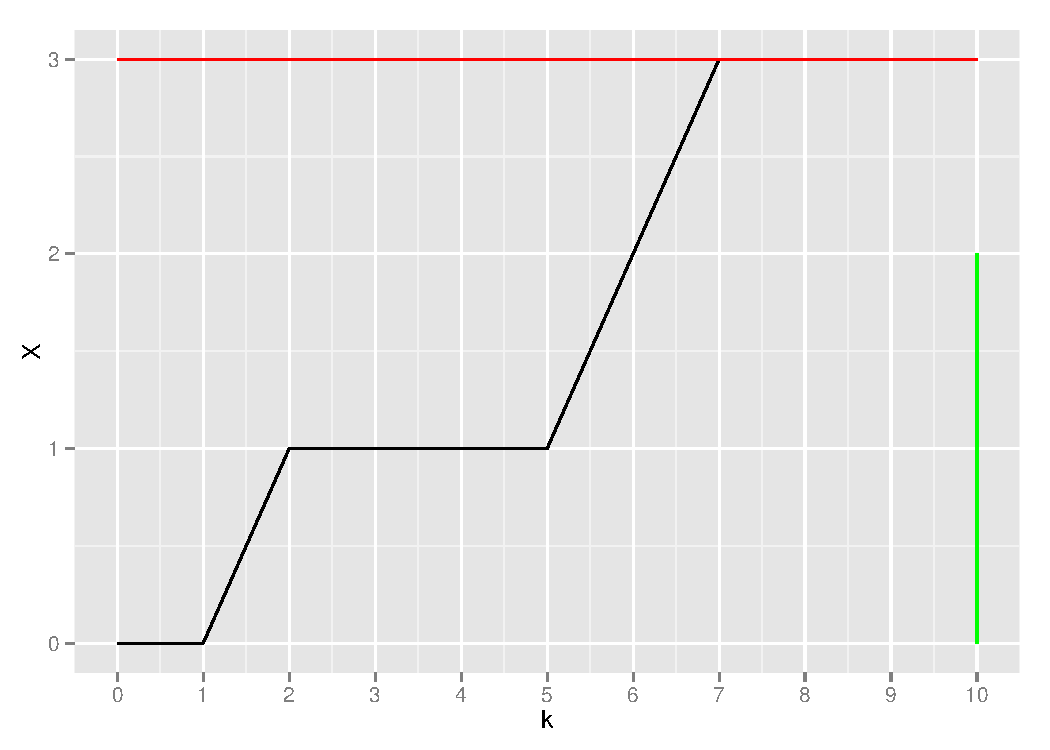
\includegraphics[width=\textwidth]{BernoulliProcess.pdf}
\caption{
A realization of the stopped process with $p=0.3$, $s=3$, and $t=10$.
The red line segment indicates the stopping boundary defined by $s$ and 
the green line segment indicates the stopping boundary defined by $t$.
}
\label{fig:bp}
\end{figure}

\begin{prop} \label{prop:sandt}
Let $X_\mathcal{S}$ refer to the stopped process described above, which
is parameterized by $p$, $s$, and $t$.  
If $s > t$ then 
$X_\mathcal{S}(k') < s$ for all $0 \leq k' \leq t$; the process will never
reach $s$. 
\end{prop}
\begin{proof}
First, note that $X_\mathcal{S}(k') \leq X(k')$ for all $0 \leq k' \leq t$.
Second, note that $X(k') \leq t$ since the process
is non-decreasing and increases by a maximum of one at each step.
Since $s > t$ by assumption $X(k')$ must also be less than $s$.
\end{proof}

\begin{prop}
Let $\tau = \min\{ k: \{X_\mathcal{S}(k) = s\} \vee \{k \geq t\} \}$ be 
the stopping time for $\mathbf{X_\mathcal{S}}$. The support of the 
stopping time is
$\{ s \leq \tau \leq t \}$ when $s \leq t$ and $\{\tau = t\}$ otherwise.
\end{prop}
\begin{proof}
$\{\tau > t \} = 0$ holds since 
\begin{align*}
\tau &\leq \min\{k : \{k \geq t\} \} \\
  & = t.
\end{align*}
If $s \leq t$ then 
$X_\mathcal{S}(k') \leq k'$ for all $0 \leq k' \leq t$, which implies
that $X_\mathcal{S}(k'') < s$ for all $k'' < s$, and $\{\tau < s\} = 0$. 
If $s \geq t$, then 
\begin{align*}
\tau &= \min\{k : \{X_\mathcal{S}(k) = s\} \vee \{k \geq t\} \} \\
  & = \min\{k : \{k \geq t\} \} \\
  & = t
\end{align*}
since $X_\mathcal{S}(k) < s$ as a consequence of Proposition \ref{prop:sandt}.
\end{proof}

\begin{prop}
Let
\begin{equation*}
N(k, p, s) = {k-1 \choose s-1} p^s q^{k-s}
\end{equation*}
be the Negative Binomial distribution, then the density function for $\tau$ is
\begin{equation*}
f_\tau(k, p, s, t) =  \{s \leq k < t\} N(k, p, s) + 
  \{k=t\} \left( 1 - \sum_{i=s}^{t-1} N(i, p, s) \right).
\end{equation*}
\end{prop}
\begin{proof}
TODO: Write the proof
\end{proof}

%\begin{prop}
%Equation \ref{eqn:tail} can equivalently be written as
%\begin{equation*}
%T(k, p, s, t) = \sum_{i=0}^{s-1} {t \choose i} p^i q^{t-i}.
%\end{equation*}
%\end{prop}
%\begin{proof}
%TODO: Write the proof
%\end{proof}


%From Proposition \ref{prop:sandt}, the process cannot hit $s$ until at 
%least $s$ steps and therefore $\{\tau < s\} =0$. For any other value 
%$\{s \leq \tau \leq t\}$ there
%is a non-zero probability that the processes can be stopped as long as
%$0 < p < 1$ and $s < t$. If $s \geq t$ then the process stops at $t$ 
%almost surely.

\section*{The Stopped Negative Binomial Distribution}

In the last section $t$, the maximum time that the process would
run without stopping, was a constant integer value. Now consider 
the case where a function of $X_\mathcal{S}$, $k$, and $t$
\begin{equation*}
\psi(\Xs, k, t) = \min\{k: \Xs(k) = k - t \}.
\end{equation*}
This change to the model limits the number of unsuccessful coin flips
in $\Xs$ to $t$. The process can be conceptualized as a series of coin
flips that stops when either $s$ heads or $t$ tails are reached. This
new process, which will be referred to as the Stopped Negative Binomial
Process, can be conceptualized in one of two ways. First, it can be thought of
as a walk on the integers, starting at the origin. At each step a coin is 
flipped. If it is heads then one step is taken in the positive direction 
on the vertical axis. Otherwise, a step is taken in the positive direction
on the horizontal axis. The walk stops when either $s$ is reached on the
vertical axis or $t$ is reached on the horizontal axis. A visual example 
is shown in Figure \ref{fig:zelterman_viz}.

\begin{figure}[ht]
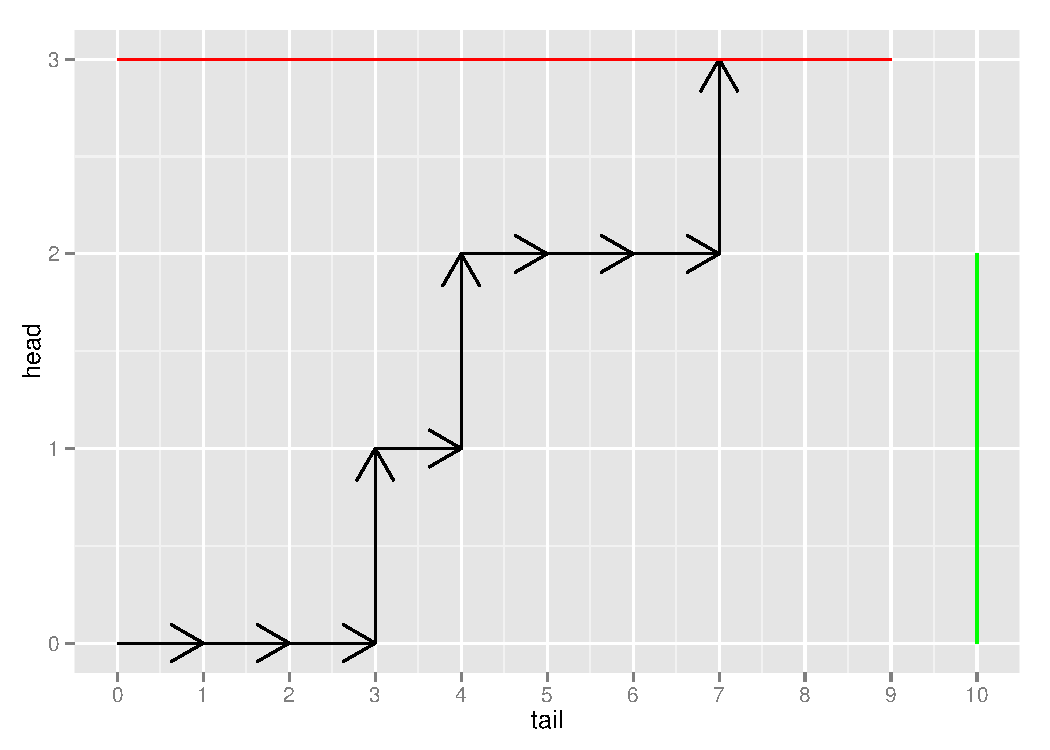
\includegraphics[width=\textwidth]{ZeltermanPlot.pdf}
\caption{
A realization of the Stopped Negative Binomial Process with $p=0.3$, $s=3$, 
and $t=10$. An arrow to the right indicates a coin flip of ``tails'' and
an arrow in the vertical direction indicates ``heads.''
}
\label{fig:zelterman_viz}
\end{figure}

Second, the process can be visualized in a manner similar to 
Figure \ref{fig:bp}. At each
step a coin is flipped. If it is heads, the process advances one diagonally
in the positive horizontal and vertical direction. Otherwise, it advances
in the positive horizontal direction only. The difference between the Stopped
Negative Binomial Process and the one from the previous section being that
the boundary defined by $t$ is dependent on $\Xs$, $k$, and $t$. A visual
example is shown in Figure \ref{fig:kane_viz}.

\begin{figure}[ht]
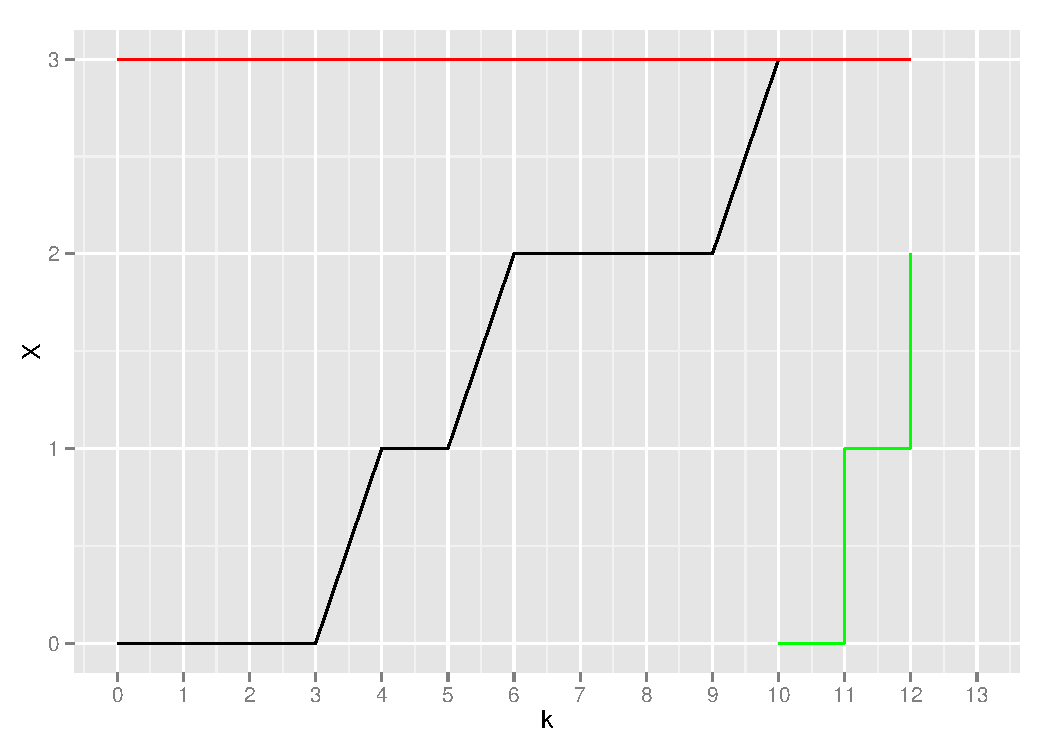
\includegraphics[width=\textwidth]{KanePlot.pdf}
\caption{
The same process shown in Figure \ref{fig:zelterman_viz} but shown as
a process where the horizontal axis denotes time and the vertical axis
denotes the number of ``heads.'' 
}
\label{fig:kane_viz}
\end{figure}

\begin{prop}
The distribution of the stopping time of the Stopped Negative Binomial Process 
is 
\begin{equation*}
f_N(k, p, s, t) = \alpha \{s \leq k \leq s+t\} N(k, p, s) + 
  \beta \{t \leq k \leq s+t-1 \} R(k, p, t).
\end{equation*}
where 
\begin{align*}
&R(k, p, t) = {k-1 \choose k-t} p^{k-t} q^t, \\
&\alpha = \frac{\sum_{i=s}^t N(i, p, s)}
  {\sum_{i=s}^t N(i, p, s) + \sum_{i=t}^{s+t-1} R(i, p, t)}, \\
&\beta = 1 - \alpha
\end{align*}

\end{prop}
\begin{proof}
\end{proof}

\begin{prop}
TODO: the ``peeking property''
\end{prop}
\begin{proof}
\end{proof}



\end{document}

